\documentclass[a4paper, 10pt, ]{article}

\usepackage[slovak]{babel}

\usepackage[utf8]{inputenc}
\usepackage[T1]{fontenc}

\usepackage[left=4cm,
			right=4cm,
			top=2.1cm,
			bottom=2.6cm,
			footskip=7.5mm,
			twoside,
			marginparwidth=3.5cm,
			%showframe,
			]{geometry}

\usepackage{graphicx}
\usepackage{xcolor}

% ------------------------------

\usepackage{lmodern}

\usepackage[tt={oldstyle=false,proportional=true,monowidth}]{cfr-lm}

% ------------------------------

\usepackage{amsmath}
\usepackage{amssymb}
\usepackage{amsthm}

\usepackage{booktabs}
\usepackage{multirow}
\usepackage{array}
\usepackage{dcolumn}

\usepackage{natbib}

\usepackage[singlelinecheck=true]{subfig}


% ------------------------------


\usepackage{sectsty}
\allsectionsfont{\sffamily}


\usepackage{titlesec}
\titleformat{\paragraph}[hang]{\sffamily  \bfseries}{}{0pt}{}
\titlespacing*{\paragraph}{0mm}{3mm}{1mm}


\usepackage{fancyhdr}
\fancypagestyle{plain}{%
\fancyhf{} % clear all header and footer fields
\fancyfoot[C]{\sffamily {\bfseries \thepage}\ | {\scriptsize\oznacenieCasti}}
\renewcommand{\headrulewidth}{0pt}
\renewcommand{\footrulewidth}{0pt}}
\pagestyle{plain}


% ------------------------------


\makeatletter

	\def\@seccntformat#1{\protect\makebox[0pt][r]{\csname the#1\endcsname\hspace{5mm}}}

	\def\cleardoublepage{\clearpage\if@twoside \ifodd\c@page\else
	\hbox{}
	\vspace*{\fill}
	\begin{center}
	\phantom{}
	\end{center}
	\vspace{\fill}
	\thispagestyle{empty}
	\newpage
	\if@twocolumn\hbox{}\newpage\fi\fi\fi}

	\newcommand\figcaption{\def\@captype{figure}\caption}
	\newcommand\tabcaption{\def\@captype{table}\caption}

\makeatother


% ------------------------------


\def\naT{\mathsf{T}}

\hyphenpenalty=6000
\tolerance=1200


% ------------------------------


\usepackage[pdfauthor={MT},
			pdftitle={AR},
			pdfsubject={},
			pdfkeywords={},
			hidelinks,
			breaklinks,
			]{hyperref}



% ------------------------------

\usepackage{enumitem}





\usepackage[titles]{tocloft}

\setlength{\cftsecindent}{-12mm}
\setlength{\cftsecnumwidth}{12mm}
\renewcommand{\cftsecpresnum}{\hfill}
\renewcommand{\cftsecaftersnum}{\hspace{4mm}}

\setlength{\cftsubsecindent}{-12mm}
\setlength{\cftsubsecnumwidth}{12mm}
\renewcommand{\cftsubsecpresnum}{\hfill}
\renewcommand{\cftsubsecaftersnum}{\hspace{4mm}}

\setlength{\cftsubsubsecindent}{-12mm}
\setlength{\cftsubsubsecnumwidth}{12mm}
\renewcommand{\cftsubsubsecpresnum}{\hfill}
\renewcommand{\cftsubsubsecaftersnum}{\hspace{4mm}}

\renewcommand{\cftsecpagefont}{\lstyle \bfseries}
\renewcommand{\cftsubsecpagefont}{\lstyle}
\renewcommand{\cftsubsubsecpagefont}{\lstyle}


% ------------------------------





\graphicspath{{fig/}{PY/fig/}}


\def\oznacenieCasti{AR02 - LS2021}





\begin{document}

\lstset{%
style=mystyle,
rangebeginprefix=\#\#\#\ cellB\ ,%
rangebeginsuffix=\ \#\#\#,%
rangeendprefix=\#\#\#\ cellE\ ,%
rangeendsuffix=\ \#\#\#,%
includerangemarker=false,
}



\fontsize{12pt}{22pt}\selectfont

\centerline{\textsf{Adaptívne riadenie} \hfill \textsf{\oznacenieCasti}}

\fontsize{18pt}{22pt}\selectfont





\begin{flushleft}
	\textbf{\textsf{O adaptívnej stabilizácii}}
\end{flushleft}





\normalsize

\bigskip

{\hypersetup{hidelinks}

\tableofcontents

}

\bigskip

\vspace{18pt}











\section{Cvičenie prvé}
\label{cvprve}


\begin{enumerate}[leftmargin=0pt, labelsep=3mm, itemsep=0pt]

	\item  Uvažujme riadený systém v tvare
	\begin{equation}
		\dot{x}(t) = a\, x(t) + b \, u(t) \label{sustavaNaCv}
	\end{equation}
	kde $x(t)$ je stavová veličina sytému, $u(t)$ je akčný zásah (výstup) regulátora. Parameter $b = 1$ a parameter $a$ je neznáma konštanta.
    \begin{itemize}
		\item Koľkého rádu je systém \eqref{sustavaNaCv}?
		\item Aká je prenosová funkcia daného dynamického systému?
		\item Aký je charakteristický polynóm a charakteristická rovnica dynamického systému?
		\item Aké sú korene charakteristického polynómu?
		\item Pre ktoré $a$ je systém stabilný a pre ktoré $a$ je nestabilný? Nájdite intervaly.
		\item Aké je zosilnenie sústavy? Aké sú časové konštanty?
		\item Ktorého reálneho systému (napríklad), je vhodným modelom takáto sústava?
	\end{itemize}

	\item Zostavte simulačnú schému systému \eqref{sustavaNaCv}. Zvoľte konkrétnu hodnotu parametra $a$~z~nájdeného intervalu tak aby riadený systém \eqref{sustavaNaCv} bol stabilný. Nech začiatočný stav je $x(0) = 1$ a~$u(t)=0$. Simuláciou (pre vhodný časový úsek) ukážte, že $x = 0$ je rovnovážny stav sústavy.

	\item Nech začiatočný stav sústavy $x(0) = 1$. Zvoľte konkrétnu hodnotu parametra $a$~tak aby sústava \eqref{sustavaNaCv} bola \textbf{nestabilná}. Spustite simuláciu a pozorujte nestabilný priebeh stavovej veličiny. Pridajte k riadenému systému regulátor daný nasledovne:
	\begin{equation}
		u = -k\, x \qquad k > \left| a \right|
	\end{equation}
	a overte, že URO je stabilný. Vysvetlite. Vyskúšajte rôzne hodnoty zosilnenia $k$.

	\item Nech začiatočný stav sústavy $x(0) = 1$. Zvoľte konkrétnu hodnotu parametra $a$~tak aby sústava \eqref{sustavaNaCv} bola \textbf{nestabilná}. Pridajte k riadenému systému regulátor daný nasledovne:
	\begin{equation}
		u = -k\, x; \qquad \dot{k} = x^2
	\end{equation}
	Simuláciou vyšetrite stabilitu URO.

	\item Overte, že regulátor z predchádzajúcej úlohy zabezpečí stabilizáciu URO pre rôzne hodnoty $a$ a rôzne hodnoty začiatočného stavu $x(0)$ (vyskúšajte rôzne). Teda regulátor je adaptívny! Vysvetlite\ldots

\end{enumerate}




\section{Viac k téme cvičenia prvého}

Zaoberáme sa systémom, ktorého vhodným modelom je diferenciálna rovnica v tvare
\begin{equation} \label{viac_riadsys}
	\dot x(t) = a x(t) + u(t)
\end{equation}
kde $x(t)$ je výstupná veličina, $u(t)$ je vstupná veličina a konštanta $a$ je parameter riadeného systému.

Nech je známe, že riadený systém je nestabilný. To znamená, že parameter $a$ je kladné číslo. Nie je známa hodnota parametra $a$, ale je známe jeho znamienko. Keďže riadený systém je nestabilný, po vychýlení z rovnovážneho stavu (rovnovážnej polohy) sa výstupná veličina nevráti na hodnotu v rovnovážnom stave.

Úlohou je navrhnúť taký riadiaci systém, ktorý zabezpečí, že výstupná veličina sa vráti na hodnotu v rovnovážnom stave napriek tomu, že jej začiatočná hodnota (začiatočný stav) je iná ako v rovnovážnom stave. Teda začiatočný stav riadeného systému je vychýlený z rovnovážneho stavu.



\bigskip

\noindent
Mimochodom, rovnica \eqref{viac_riadsys} je dynamický systém, lineárny systém a rád systému je 1 (lineárny dynamický systém 1. rádu). Z toho vyplýva, že v rovnovážnom stave je hodnota výstupu $y(t)$ nulová.

Diferenciálnu rovnicu \eqref{viac_riadsys} je možné (pri uvažovaní nulových začiatočných podmienok) previesť do tvaru prenosovej funkcie. Ak sa uváži, že
\begin{equation}
	s x = a x + u
\end{equation}
kde $s$ je Laplaceov operátor, pričom tu plní funkciu časovej derivácie, potom možno písať
\begin{subequations}
	\begin{align}
		s x - a x &= u \\
		\left( s - a \right) x &= u \\
		\frac{x}{u} &= \frac{1}{\left( s - a \right)}
	\end{align}
\end{subequations}
čo je prenosová funkcia zodpovedajúca systému \eqref{viac_riadsys}. Charakteristický polynóm je $\left( s - a \right)$ a koreňom tohto polynómu je (číslo) $a$. Keďže je známe, že systém je nestabilný, potom pól systému, teda koreň charakteristického polynómu leží v pravej polrovine komplexnej roviny. To znamená, že $a>0$.

% \bigskip



\begin{figure}[!t]
	\centering
	\makebox[\textwidth][c]{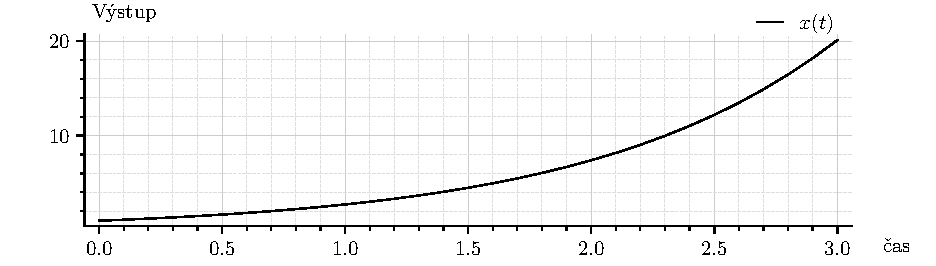
\includegraphics{figsc_ar02_fig00_0.pdf}}
	\caption{Výsledok numerickej simulácie systému \eqref{viac_riadsys} pre $a = 1$ pri začiatočnom stave $x(0) = 1$.}
	\label{Výsledok numerickej simulácie systému}
\end{figure}


\paragraph{Samotný riadený systém}

\noindent
S využitím numerickej simulácie ukážme, že systém \eqref{viac_riadsys} je pre $a>0$ nestabilný. Pri tomto overení je vstupná veličina systému $u(t)$ nepodstatná. Preto je nastavená na nulovú hodnotu. Nech začiatočná hodnota stavovej veličiny $x(0) = 1$ a nech hodnota parametra $a = 1$. Simulujme 3 časové jednotky. Výsledok numerickej simulácie  je na obr.~ \ref{Výsledok numerickej simulácie systému}.






\paragraph{Formalizácia požiadaviek na kvalitu riadenia}

Úlohou je aby sa výstupná veličina vrátila na nulovú hodnotu (do rovnovážneho stavu). Ale ako rýchlo sa tam má vrátiť? Aké sú požiadavky na prechodný dej pri činnosti riadiaceho systému?

Nech sú tieto požiadavky premietnuté do akéhosi vzorového dynamického systému, ktorý má stavovú veličinu $x_m(t)$. Tento vzorový systém je
\begin{equation} \label{viac_refmodel}
	\dot x_m(t) = -a_m x_m(t)
\end{equation}
Jeho parametrom je $a_m$. Ak bude $a_m > 0$, potom bude tento systém stabilný a~teda vždy sa ustáli v rovnovážnom stave, to je v tomto prípade samozrejme nula. Pól systému je $-a_m$. Voľbou pólu sa volí dynamika s akou sa systém bude vracať do rovnovážneho stavu. Tento vzorový systém teda zodpovedá úlohe, ktorú máme, a~navyše úplne presne špecifikuje akékoľvek iné požiadavky, ktoré nemusia priamo plynúť zo zadania úlohy.


\paragraph{Teoretická existencia ideálneho riadiaceho systému}

Od riadiaceho systému chceme aby pre riadený systém \eqref{viac_riadsys} zabezpečil, že výstupná veličina riadeného systému \eqref{viac_riadsys} $x(t)$ sa bude správať práve tak ako veličina $x_m(t)$. V~ideálnom prípade je teda odchýlka $e(t) = x(t) - x_m(t)$ nulová. Je vôbec možné zostaviť taký riadiaci systém?

Uvažujme nasledujúci predpis pre výpočet hodnoty akčného zásahu $u(t)$.
\begin{equation} \label{viac_idealZR}
	u(t) = -k^* x(t)
\end{equation}
Zovšeobecnene budeme takýto predpis nazývať zákon riadenia. Predpisuje ako sa vypočíta akčný zásah. Zákon riadenia obsahuje dva prvky. Signál $x(t)$, ktorý je spätnou väzbou od riadeného systému, keďže $x(t)$ je výstupom riadeného systému, a druhým prvkom zákona riadenia je parameter $k^*$.


Dosaďme za $u(t)$ v riadenom systéme. Získa sa tak rovnica uzavretého regulačného obvodu (URO). V tomto prípade v tvare
\begin{subequations}
	\begin{align}
		\dot x(t) &= a x(t) - k^* x(t) \\
		\dot x(t) &= \left( a - k^* \right) x(t)
	\end{align}
\end{subequations}
Pripomeňme, že je žiadané aby odchýlka $e(t) = x(t) - x_m(t)$ bola nulová. Je zrejmé, že ak by platilo $\left( a - k^* \right) = -a_m$, potom
\begin{align}
	\dot x(t) = -a_m x(t)
\end{align}
URO a uvedený vzorový systém \eqref{viac_refmodel} by teda mali úplne rovnaký predpis (rovnakú rovnicu). Samozrejme, v URO vystupuje signál $x(t)$ a vo vzorovom systéme vystupuje signál $x_m(t)$. Inak sú však tieto dva systémy úplne rovnaké. To znamená, že možno písať $x(t) = x_m(t)$ a teda daná celková úloha je splnená.

Týmto sa ukázalo, že je možné zostaviť taký riadiaci systém, teda nájsť taký zákon riadenia, ktorý rieši danú úlohu.

V tomto prípade sme našli zákon riadenia \eqref{viac_idealZR}, ku ktorému prislúcha tzv. podmienka zhody, čo v tomto prípade je
\begin{equation}
	\left( a - k^* \right) = -a_m
\end{equation}
Ide o podmienku zhody medzi URO a istým vzorovým systémom, ktorý sa vo všeobecnosti nazýva Referenčný model (RM). RM predpisuje ako sa má správať URO.

Pre riešenie úlohy tohto typu teda v prvom rade musí existovať \emph{podmienka zhody} čo je, pochopiteľne, istá rovnica a táto rovnica musí byť riešiteľná. Neznámou je samozrejme parameter zákona riadenia. V tomto prípade $k^*$. Teoretické riešenie je
\begin{subequations}
	\begin{align}
		 a - k^* &= -a_m \\
		 k^* &= a_m + a
	\end{align}
\end{subequations}
Konkrétnu hodnotu parametra $k^*$ však nevieme určiť pretože nepoznáme konkrétnu hodnotu parametra $a$. Ale vieme, že vôbec existuje ideálne $k^*$. To je veľmi, veľmi dôležité!













\paragraph{Zákon riadenia s premenlivým parametrom}

Zákon riadenia \eqref{viac_idealZR}, ktorý má konštantný parameter $k^*$, teda nevieme použiť, pretože nevieme vypočítať $k^*$. Zachovajme ale štruktúru zákona riadenia (aby stále existovali riešiteľné podmienky zhody) a neznámy parameter $k^*$ nahraďme parametrom, ktorému dovolíme meniť sa v čase. Adaptovať sa. Adaptovať sa tak, aby sme splnili úlohu. Adaptívny zákon riadenia nech teda je
\begin{equation} \label{adapt_idealZR}
	u(t) = -k(t) x(t)
\end{equation}
kde $k(t)$ je časovo premenlivý parameter.

Parameter $k(t)$ sa vlastne môže meniť akokoľvek. Cieľom však je splnenie úlohy. To znamená, že ideálne $e(t) = x(t) - x_m(t) = 0$. To si však vyžaduje mať možnosť určiť $k^*$. Žiadať teda $e(t) = 0$ v tomto prípade nikam nevedie. Žiadajme ale aby $e(t) \to 0$, teda že odchýlka $e(t)$ sa asymptoticky blíži k nule. Pritom sa však nevylučuje aby mohla byť aj nulová.

Ak $e(t) \to 0$ potom vlastne $x(t) \to x_m(t)$, teda signál $x(t)$ sa hodnotou približuje k~signálu $x_m(t)$. Aká je vlastne hodnota signálu $x_m(t)$? Predpisuje ju referenčný model \eqref{viac_refmodel}. K rovnici \eqref{viac_refmodel} chýba explicitne napísaná začiatočná podmienka pre signál $x_m(t)$, teda $x_m(0)$. Úlohou je aby sa $x(t)$ dostalo do rovnovážneho stavu. Teda do nuly. Signál $x_m(t)$ by teda mal byť nulový. A prečo nie hneď aj od začiatku? Nech teda $x_m(0) = 0$. Potom vzhľadom na rovnicu \eqref{viac_refmodel} je $x_m(t) = 0$ po celý čas! Ak teda chceme $e(t) \to 0$, potom máme $x(t) \to 0$. Alebo inak povedané  $e(t) = x(t) - x_m(t) = x(t) - 0$. Teda $e(t) = x(t)$.










\paragraph{Spôsob ako meniť (adaptovať) parameter zákona riadenia}

Stále však nie je zrejmé ako adaptovať (meniť) parameter $k(t)$ tak aby sme splnili modifikovanú požiadavku $e(t) \to 0$.

URO s adaptívnym zákonom riadenia \eqref{adapt_idealZR} je
\begin{align}
	\dot x(t) &= \left( a - k(t) \right) x(t) \qquad x(0) \neq 0
\end{align}
Ak by platilo $\left( a - k(t) \right) < 0$, potom by bol URO stabilný a $x(t) \to 0$ pri akejkoľvek začiatočnej hodnote $x(0)$. A to je presne požiadavka pre splnenie úlohy. Hodnota parametra $a$ je však neznáma, ale je zrejmé, že ak bude $k(t)$ dostatočne veľké (vzhľadom na $a$), potom celý výraz $\left( a - k(t) \right)$ bude záporný.

Ako však získať informáciu o tom kedy je $k(t)$ dostatočne veľké? Ak nie je dostatočne veľké, potom je vo všeobecnosti odchýlka $e(t)$ nenulová! Teda pri nenulovej $e(t)$ treba $k(t)$ meniť (v čase), konkrétnejšie, treba zvyšovať jeho hodnotu. Len ak by platilo, že $e(t) = 0$, len vtedy možno prestať meniť $k(t)$.

Zmena parametra $k(t)$ v čase je jeho časová derivácia $\dot k(t)$.

Pre vzťah
\begin{equation} \label{viac_intuitZA}
	\dot k(t) = e^2(t)
\end{equation}
platí, že ak je $e(t)$ nenulové, tak zmena $k(t)$ je kladná, a len ak $e(t) = 0$ aj zmena $k(t)$ je nulová. Pomocou tohto predpisu pre $\dot k(t)$ teda dosiahneme také zmeny $k(t)$ v čase, aké sú potrebné pre dosiahnutie $x(t) \to 0$ a teda $e(t) \to 0$, čo je splnenie stanoveného cieľa!

Rovnica \eqref{viac_intuitZA} predpisuje ako sa má meniť parameter zákona riadenia tak aby bol cieľ riadenia splnený. Vo všeobecnosti sa takýto predpis nazýva zákon adaptácie.

Mimochodom, keďže vieme, že v tomto prípade platí $e(t) = x(t)$, potom \eqref{viac_intuitZA} možno písať aj v tvare
\begin{equation} \label{viac_praktickyZA}
	\dot k(t) = x^2(t)
\end{equation}
ba dokonca aj
\begin{equation}
	\dot k(t) = e(t)x(t)
\end{equation}
čo by bol pre skúsenejšieho v tejto oblasti azda najvhodnejší zápis. V tomto prípade praktickejším je tvar \eqref{viac_praktickyZA}, pretože si to nevyžaduje žiadny ďalší signál, len $x(t)$, ktorý je samozrejme k dispozícii.


\paragraph{Overenie adaptívneho riadiaceho systému}

Zákon adaptácie \eqref{viac_praktickyZA} teraz dopĺňa zákon riadenia \eqref{adapt_idealZR}. K uvedenému ešte pre úplnosť prislúcha aj referenčný model čo však v tomto prípade možno zanedbať. Tieto súčasti spolu tvoria adaptívny riadiaci systém, ktorý spĺňa danú úlohu.

S využitím numerickej simulácie ukážme, že uvedený adaptívny riadiaci systém stabilizuje riadený systém, t.j. pri začiatočnom stave mimo rovnovážneho stavu zabezpečí asymtotické približovanie sa výstupu riadeného systému k rovnovážnemu stavu. Na obr.~\ref{Výsledok numerickej simulácie adapt systému} sú výsledky použitia tohto adaptívneho riadiaceho systému pre prípad keď je v riadenom systéme $a = 1$ a $x(0) = 1$. Je možné pozorovať vyššie uvedené predpoklady a teda, že parameter $k(t)$ sa zvyšuje až pokým neprekročí hodnotu parametra $a$. Vtedy sa URO stane stabilným a jeho stavová veličina sa z hodnoty, ktorú práve má, prirodzene začne vracať do rovnovážneho stavu, teda na hodnotu nula. Ďalej rýchlosť zmeny parametra $k(t)$ klesá až sa napokon ustáli. Ustáli sa na hodnote vyššej ako je hodnota parametra~$a$.

Ten istý adaptívny riadiaci systém sa bude, samozrejme, správať kvalitatívne rovnako pre rôzne hodnoty parametra riadeného systému $a$ (a pre rôzne začiatočné stavy riadeného systému). Na obr.~\ref{Výsledok numerickej simulácie adapt systému pripady} sú pre ilustráciu znázornené rôzne prípady hodnoty parametra $a$. Tým je prezentovaná schopnosť adaptácie uvedeného riadiaceho systému.


\begin{figure}[!t]
	\centering
	\makebox[\textwidth][c]{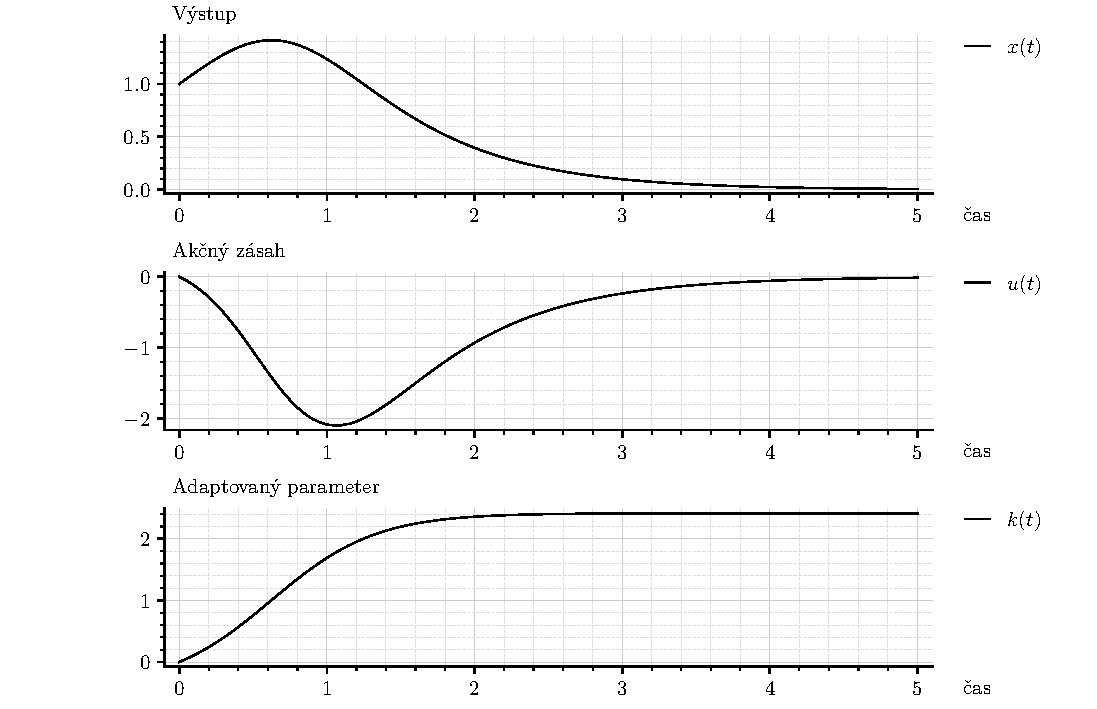
\includegraphics{figsc_ar02_fig01_0.pdf}}
	\caption{Výsledok numerickej simulácie adaptívneho riadiaceho systému pre $a = 1$ pri začiatočnom stave $x(0) = 1$.}
	\label{Výsledok numerickej simulácie adapt systému}
\end{figure}


\begin{figure}[!t]
	\centering
	\makebox[\textwidth][c]{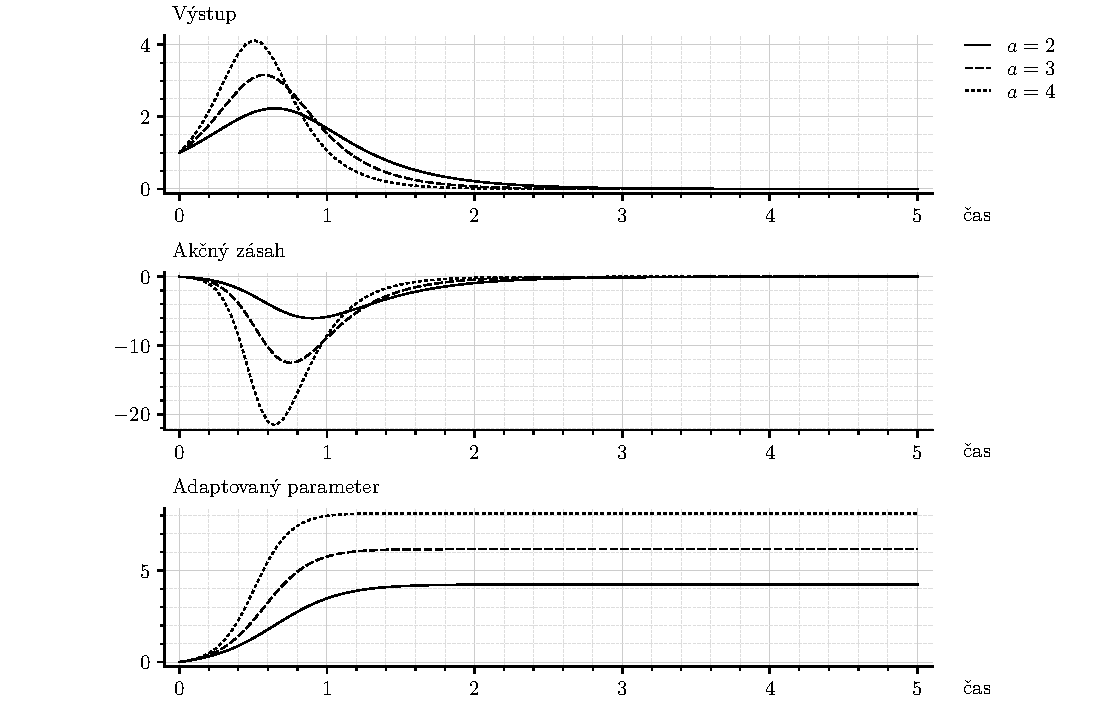
\includegraphics{figsc_ar02_fig02_0.pdf}}
	\caption{Výsledok simulácie adaptívneho riadiaceho systému pre rôzne hodnoty parametra $a$. Začiatočný stav riadeného systému je v každom prípade $x(0) = 1$.}
	\label{Výsledok numerickej simulácie adapt systému pripady}
\end{figure}













\section[Formálny opis adaptívnej stabilizácie pre systém 1.~rádu]{Formálny opis adaptívnej stabilizácie\\pre systém 1.~rádu}



Nasledujúci jednoduchý príklad ilustruje situáciu, v~ktorej neznalosť hodnoty parametra riadeného systému znemožňuje návrh riadiaceho systému. Adaptívne riadenie rieši tento problém a~umožňuje navrhnúť riadiaci systém, ktorý zabezpečí splnenie cieľa riadenia pre akúkoľvek hodnotu neznámeho parametra sústavy.

Uvažujme riadený systém v tvare
\begin{equation} \label{DRsustavy}
	\dot{x} = a\, x + u
\end{equation}
kde $x(t)$ je stavová veličina systému, $u(t)$ je akčný zásah (výstup) regulátora a~parameter $a$ je neznáma konštanta. Rovnovážny bod systému je v~bode $x=0$. Cieľom riadenia je aby stavová veličina $x$ bola asymptoticky stabilná, teda aby po vychýlení stavu $x$ z~rovnovážneho bodu sa stav postupne približoval (asymptoticky) naspäť k~rovnovážnemu bodu.  To platí pre nasledujúci systém:
\begin{equation} \label{DRstabSustavy}
	\dot{x} = -a_m\, x
\end{equation}
kde konštanta $a_m > 0$.

Ak by bol parameter $a$ známy, potom lineárny regulátor v tvare
\begin{equation} \label{skalarnyZakonRiadenia}
	u = -k\, x \qquad k > \left| a \right|
\end{equation}
zabezpečí splnenie úlohy. V takomto prípade nezáleží, či samotný riadený systém (bez riadenia, $u=0$) stabilný je alebo nie je. Poznáme absolútnu hodnotu $\left| a \right|$ a zosilnenie $k$ zvolíme väčšie ako $\left| a \right|$. Potom je zrejmé, že
\begin{equation} \label{DRURO}
	\dot{x} = a\, x + \left( -k\, x \right) = \left(a-k\right)\,x
\end{equation}
je rovnica uzavretého regulačného obvodu (URO) spĺňajúceho cieľ riadenia, pretože v najhoršom (hraničnom) prípade, kedy URO je stabilný, nie však asymptoticky stabilný, ak $k = \left| a \right|$ platí $\left(a-\left| a \right|\right) \leq 0$ pre každé $a$.

Pre návrh regulátora \eqref{skalarnyZakonRiadenia} v podstate stačí poznať horné ohraničenie parametra $a$.

Na druhej strane, parameter $a$ sa môže s časom meniť a jeho horná hranica nemusí byť známa. Pre nevhodne zvolené $k$ potom môže nastať situácia $a>k>0$. Vtedy URO je nestabilný. Pre neznámu hornú hranicu parametra $a$ nie je možné navrhnúť riadiaci systém, ktorý vždy zabezpečí splnenie úlohy riadenia --- stabilný URO.

Riešenie tejto úlohy metódami Adaptívneho riadenia, ktoré budú popísané podrobne neskôr, vedie na nasledovné:

Riadiaci systém v tvare
\begin{equation} \label{adaptRiadiacSystem}
	u = -k\, x; \qquad \dot{k} = x^2
\end{equation}
zabezpečí, že všetky signály v URO sú ohraničené a $x$ s časom konverguje do nuly pričom \emph{nezáleží} na hodnote parametra $a$. Požiadavkou nie je presné určenie hodnoty parametra $a$, ale len stabilizácia systému. Nie je požadovaná ani presná hodnota parametra $k$. Adaptívny riadiaci systém len zabezpečí, že $k$ je ohraničené, teda stabilné. Pre tento konkrétny jednoduchý príklad je zrejmé, že $k$ sa ustáli na hodnote väčšej ako $a$, čo však nehovorí nič o presnej hodnote parametra $a$ ani $k$.

Ukážme, že riadiaci systém \eqref{adaptRiadiacSystem} stabilizuje stavovú -- výstupnú veličinu sústavy \eqref{DRsustavy}.

Najskôr upresníme cieľ riadenia. Cieľom je aby $x$~konvergovalo k~nule pre čas $t\rightarrow\infty$. Žiadanou hodnotou pre $x$ je $r=0$. Uvažujeme všeobecný (akýkoľvek) začiatočný stav $x_0$. Začiatok je v čase $t = 0$, teda: $x(0) = x_0$. Cieľ si vyžaduje aby URO bol stabilný. Preto nech želaný pól URO je $-a_m$, kde $a_m>0$ sa volí podľa požiadaviek na rýchlosť regulácie. Potom referenčný (ideálny, želaný) priebeh stavu $x$ opisuje rovnica
\begin{equation} \label{drRM}
	\dot{x}_m = -a_m\, x_m
\end{equation}
kde $x_m$ stavová veličina ideálneho URO. Je prirodzené očakávať (lepšie povedané, zvoliť si), že začiatočný stav $x_m(0) = 0$ z čoho vyplíva, že v ďalšom môžme uvažovať $x_m = 0$.

V ideálnom prípade, keď poznáme parameter $a$,~vieme určiť  pre zákon riadenia „ideálne“ $k^*$:
\begin{equation} \label{idealZakRiadenia}
	u = -k^* \, x; \qquad k^* = a + a_m
\end{equation}
Vtedy sa URO presne zhoduje s ideálnym URO, teda s~referenčným modelom \eqref{drRM}
\begin{equation}
	\begin{split}
		\dot{x} &= a\, x + \left( -k^* \, x \right) = \left(a - k^* \right)\,x = \left(a - a - a_m \right)\,x  =- a_m\,x
	\end{split}
\end{equation}
Pretože $a$ je neznáme, $k^*$ nevieme vypočítať a~zákon riadenia \eqref{idealZakRiadenia} nemôže byť použitý.

Žiadaná hodnota pre stavovú veličinu $x$ je $r = 0$ a žiadame aby sa hodnota parametra $k$ približovala k~ideálnej hodnote $k^*$ pretože len vtedy bude pól URO v~bode $-a_m$. Riadený systém vyjadríme ako funkciu ideálneho parametra $k^*$ (teda tak aby rovnica obsahovala parameter $k^*$). Tento krok má súvislosť s tým, že ide v podstate o identifikáciu parametra $k^*$ --- bližšie vysvetlenie neskôr.  Urobíme to jednoducho pripočítaním a~odpočítaním „ideálneho“ zákona riadenia \eqref{idealZakRiadenia} k~rovnici riadeného systému \eqref{DRsustavy}, potom riadený systém má tvar
\begin{equation}
	\dot{x} = a\, x - k^*\, x + k^*\, x + u
\end{equation}
Pretože $a - k^* = -a_m$ máme
\begin{equation}
	\dot{x} = -a_m\, x + k^*\, x + u
\end{equation}
Definujme tzv. \emph{adaptačnú odchýlku}. Ak adaptačná odchýlka nie je nulová je potrebné adaptovať riadiaci systém tak aby sa skutočný URO zhodoval so želaným URO. Adaptačná odchýlka má tvar
\begin{equation}
	e = x - x_m
\end{equation}
potom platí:
\begin{subequations}
	\begin{align}
		\dot{x} - \dot{x}_m &= -a_m\, x + k^*\, x + u - (-a_m)\, x  \\
		\dot{e} &= -a_m\,(x - x_m) + k^*\, x + u \\
		\dot{e} &= -a_m\,e + k^*\, x + u   \label{dynAdaptOdch}
	\end{align}
\end{subequations}
Zavedením adaptačnej odchýlky sme posunuli začiatok súradnicového systému stavového priestoru do rovnovážneho bodu riadeného systému. Inými slovami, rovnovážny stav veličiny $e$ z rovnice \eqref{dynAdaptOdch} je v začiatku stavového priestoru riadeného systému.

Uvažujeme použitie zákona riadenia v tvare $u = -k\, x$, po dosadení do \eqref{dynAdaptOdch}:
\begin{align}
	\dot{e} &= -a_m\,e + k^*\, x  -k\, x \\
	\dot{e} &= -a_m\,e - \theta\, x
\end{align}
kde sme zaviedli pojem \emph{chyba nastavenia parametrov zákona riadenia}, ktorý označíme $\theta$, a v tomto prípade $\theta = k - k^*$.

Chceme dokázať, že riadiaci systém \eqref{adaptRiadiacSystem} stabilizuje uzavretý regulačný obvod. Platí $\dot{\theta} = \dot{k} - \dot{k^*}$. Avšak $k^* = \text{konšt.}$ a teda $\dot{k^*} = 0$, preto $\dot{\theta} = \dot{k} = x^2$. Vyšetrením stability systému diferenciálnych rovníc v tvare
\begin{subequations} \label{dynamikaAdaptOdch}
	\begin{align}
		\dot{e} &= -a_m\,e - \theta\, x  \\
		\dot{\theta} &= x^2
	\end{align}
\end{subequations}
dokážeme stabilitu URO.

Zvoľme kandidáta na Ljapunovovu funkciu
\begin{equation} \label{kandLjapFcn}
	V = \frac{\left(e(t)\right)^2}{2} + \frac{\left(\theta(t)\right)^2}{2}
\end{equation}
Derivácia \eqref{kandLjapFcn} podľa času je
\begin{equation} \label{derLjapFcn}
	\dot{V} = \frac{1}{2} \, 2 \, e(t) \, \dot{e}(t) + \frac{1}{2} \, 2 \, \theta(t) \, \dot{\theta}(t) =  e(t) \, \dot{e}(t) +  \theta(t) \, \dot{\theta}(t)
\end{equation}
Do \eqref{derLjapFcn} dosadíme za $\dot{e}$ a $\dot{\theta}$, máme
\begin{subequations}
	\begin{align}
	\dot{V} &=   e \, \left( -a_m\,e - \theta \, x \right) +  \theta \, x^2 \\
	\dot{V} &=    -a_m\,e^2 - \theta\, x \, e  +  \theta \, x^2 \label{derLjapFcn2}
	\end{align}
\end{subequations}
Pretože $e = x - x_m$ a uvažujeme $x_m = 0$ a teda $e = x$, tak rovnicu \eqref{derLjapFcn2} možno písať v tvare
\begin{subequations}
	\begin{align}
		\dot{V} &=    -a_m\,x^2 - \theta\, x^2  +  \theta \, x^2 \\
		\dot{V} &=    -a_m\,x^2
	\end{align}
\end{subequations}

Pre systém \eqref{dynamikaAdaptOdch} sme našli kladne definitnú funkciu $V$ (Tá funkcia má skoro pre všetky $x$ a $\theta$ kladnú hodnotu, len pre $x=0$ a $\theta = 0$ má nulovú hodnotu. Tá nulová hodnota je práve v stacionárnom bode systému \eqref{dynamikaAdaptOdch}, ktorého stabilitu vyšetrujeme). Derivácia tejto funkcie je vo všeobecnosti záporne semidefinitná (Je rovná nule v stacionárnom -- nulovom bode, a inde môže byť len záporná alebo tiež rovná nule). Teda systém je stabilný. Presný zaver o stabilite rovnovážneho stavu systému \eqref{dynamikaAdaptOdch} v zmysle všeobecnej teórie stability podľa Ljapunova je, že rovnovážny stav je stabilný (neutrálne) podľa všetkých premenných ($x$ a $\theta$) a asymptoticky stabilný podľa premennej $x$. Prakticky to znamená, že premenná $x$ dosiahne nulovú hodnotu po skončení prechodového deja, ale premenná $\theta$ (a teda aj $k$) len konečnú hodnotu. Tým sme ukázali vlastnosti, ktoré zabezpečí \emph{adaptívny} riadiaci systém \eqref{adaptRiadiacSystem}.









\section{Otázky a úlohy}
% \addcontentsline{toc}{section}{Otázky a úlohy}

\begin{enumerate}[leftmargin=0pt, labelsep=3mm, itemsep=0pt]

	\item Vyšetrite stabilitu systému
	\begin{align*}
		\dot{e}(t) &= -a_m\,e(t) + \theta(t) \, x(t)  \\
		\dot{\theta}(t) &= -e(t) x(t)
	\end{align*}
	kde $a_m > 0$.

\end{enumerate}







\section{Príklad realizácie niektorých úloh cvičenia prvého}

Konkrétne v tejto časti sa budeme venovať najmä numerickému riešeniu diferenciálnych rovníc (ktoré vystupujú v našom cvičení prvom) s využitím, pochopiteľne, ODE solvera. Načrtneme však aj všeličo iné. Používa sa tu Python\footnote{Rovnako dobre by sa to dalo zostrojiť v akomkoľvek programovacom jazyku, v ktorom máme k~dispozícii ODE solver. Prípadne aj ten ODE solver by sme si naprogramovali\ldots}.





\subsection{Takpovediac základný prístup}



Uvažujme riadený systém v tvare
\begin{equation}
	\dot{x}(t) = a\, x(t) + u(t)
\end{equation}
kde $x(t)$ je stavová veličina sytému, $u(t)$ je akčný zásah (výstup) regulátora. Parameter $a$ je neznáma konštanta.

Funkcia, ktorá realizuje diferenciálnu rovnicu riadeného systému, nech je v~nasledujúcom tvare, kde sa hneď aj predpokladá, že $u(t)=0$.

{\catcode`\-=12
\lstinputlisting[language=Python,
                 caption={Súbor \lstinline{ar02_file02.py}},
                 % label={vypk01},
				 consecutivenumbers=false,
				 % linerange={34-42}
				 linerange=c01-c01,
                 ]{../../PY/ar02_file02.py}
}

Zostavme simulačnú schému pre riadený systém. Zvoľme konkrétnu hodnotu parametra $a$ tak aby riadený systém bol stabilný. Nech začiatočný stav je $x(0) = 1$ a~$u(t)=0$. Simuláciou (pre vhodný časový úsek) ukážme, že $x = 0$ je rovnovážny stav riadeného systému.

\noindent
Simulačnú schému nech realizuje nasledujúca funkcia:

{\catcode`\-=12
\lstinputlisting[language=Python,
                 caption={Súbor \lstinline{ar02_file02.py}},
                 % label={vypk01},
				 consecutivenumbers=false,
				 % linerange={48-63},
				 linerange=c02-c02,
                 ]{../../PY/ar02_file02.py}
}

\noindent
Nastavme a spustime simuláciu:

{\catcode`\-=12
\lstinputlisting[language=Python,
                 caption={Súbor \lstinline{ar02_file02.py}},
                 % label={vypk01},
				 consecutivenumbers=false,
				 linerange=c03-c03,
                 ]{../../PY/ar02_file02.py}
}

Všetko potrebné je teraz zaznamenáné v premenných  \lstinline{t_log} a \lstinline{x_log}. Nakreslime obrázok (pre prehľadnosť je kód kreslenia obrázku v samostatnom súbore a nie priamo tu v nasledujúcej bunke):

{\catcode`\-=12
\lstinputlisting[language=Python,
                 caption={Súbor \lstinline{ar02_file02.py}},
                 % label={vypk01},
				 consecutivenumbers=false,
				 linerange=c04-c04,
                 ]{../../PY/ar02_file02.py}
}

\begin{centering}

	\makebox[\textwidth][c]{%
	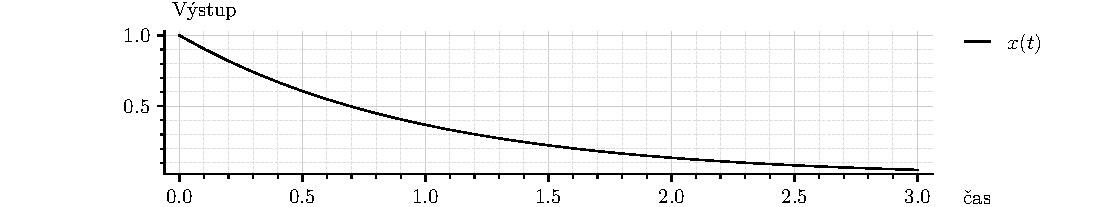
\includegraphics{figsc_ar02_fig03_0.pdf}
	}

    \vspace{-2mm}

	% \captionsetup{singlelinecheck=off}
    \figcaption{}

    \vspace{2mm}

    \label{figsc_ar02_fig03_0}

\end{centering}




\noindent
V prípade, že parameter $a$ je zvolený tak aby bol riadený systém nestabilný, výsledok je:



{\catcode`\-=12
\lstinputlisting[language=Python,
                 caption={Súbor \lstinline{ar02_file02.py}},
                 % label={vypk01},
				 consecutivenumbers=false,
				 linerange=c05-c05,
                 ]{../../PY/ar02_file02.py}
}

\begin{centering}

	\makebox[\textwidth][c]{%
	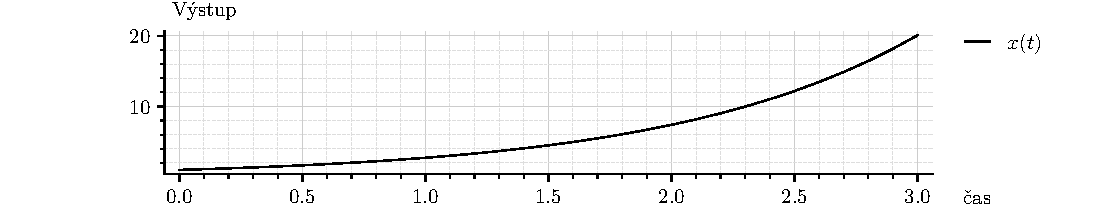
\includegraphics{figsc_ar02_fig03_1.pdf}
	}

    \vspace{-2mm}

    \figcaption{}

    \vspace{2mm}

    \label{figsc_ar02_fig03_1}

\end{centering}





Nech začiatočný stav riadeného systému je $x(0) = 1$. Ponechajme konkrétnu hodnotu parametra $a$ tak aby riadený systém bol nestabilný. Pridajme k riadenému systému riadiaci systém daný nasledovne:
	\begin{equation}
		u = -k\, x; \qquad \dot{k} = x^2
	\end{equation}
Simuláciou vyšetrime stabilitu URO.


\noindent
Funkcia, ktorá realizuje potrebné diferenciálne rovnice nech je nasledovná:


{\catcode`\-=12
\lstinputlisting[language=Python,
                 caption={Súbor \lstinline{ar02_file02.py}},
                 % label={vypk01},
				 consecutivenumbers=false,
				 linerange=c06-c06,
                 ]{../../PY/ar02_file02.py}
}

\noindent
Simulačná schéma, opäť realizovaná ako funkcia:

{\catcode`\-=12
\lstinputlisting[language=Python,
                 caption={Súbor \lstinline{ar02_file02.py}},
                 % label={vypk01},
				 consecutivenumbers=false,
				 linerange=c07-c07,
                 ]{../../PY/ar02_file02.py}
}


\noindent
Nastavenie a spustenie simulácie, pričom pripomeňme, že parameter $a$ je stále nastavený tak, aby riadený systém bol nestabilný.

{\catcode`\-=12
\lstinputlisting[language=Python,
                 caption={Súbor \lstinline{ar02_file02.py}},
                 % label={vypk01},
				 consecutivenumbers=false,
				 linerange=c08-c08,
                 ]{../../PY/ar02_file02.py}
}

\noindent
Obrázok, ktorý zobrazuje okrem výstupnej veličiny riadeného systému aj iné veličiny potrebné pre posúdenie stability celého uzavretého regulačného obvodu.


{\catcode`\-=12
\lstinputlisting[language=Python,
                 caption={Súbor \lstinline{ar02_file02.py}},
                 % label={vypk01},
				 consecutivenumbers=false,
				 linerange=c09-c09,
                 ]{../../PY/ar02_file02.py}
}



\begin{centering}

	\makebox[\textwidth][c]{%
	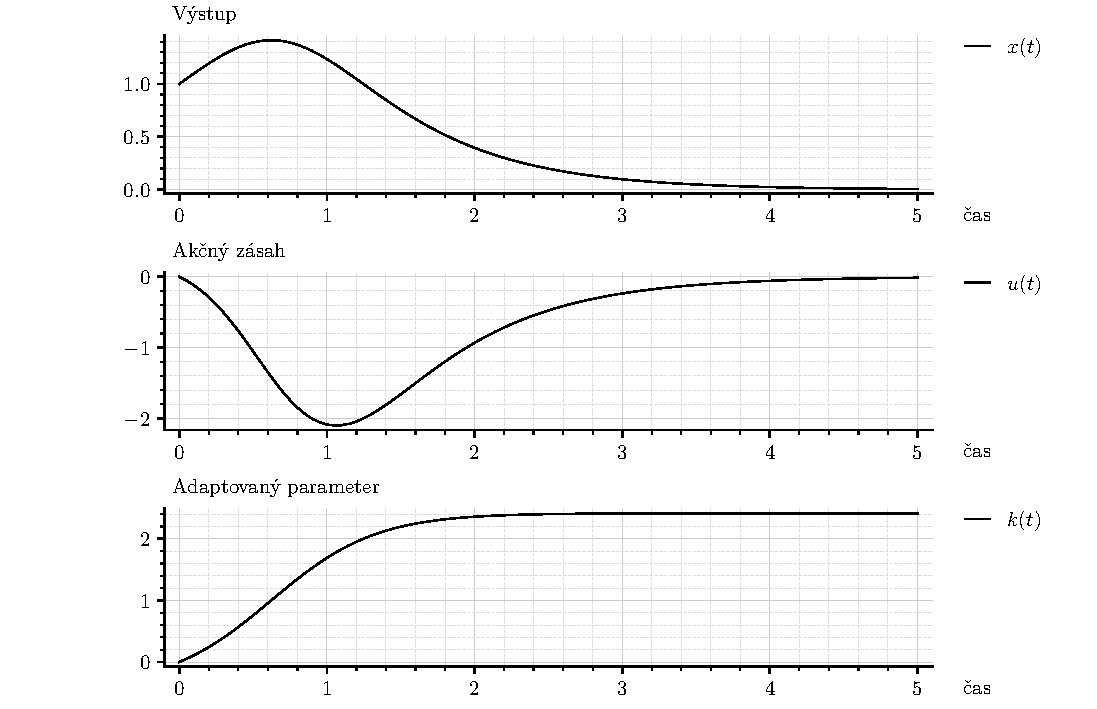
\includegraphics{figsc_ar02_fig01_1.pdf}
	}

    \vspace{-2mm}

    \figcaption{}

    \vspace{2mm}

    \label{figsc_ar02_fig01_1}

\end{centering}

\noindent
Cieľ riadenia je splnený, čo v tomto prípade znamená, že výstupná veličina sa približuje k nulovej hodnote, a všetky signály uzavretého regulačného obvodu sú ohraničené. To znamená, že URO je stabilný.

Podrobnejšia diskusia z pohľadu Adaptívneho riadenia je nad rámec konkrétne tejto časti krátkych poznámok.













\subsection{O realistickej implementácii riadiaceho systému tu uvedeného}


Uvažujme riadený systém v tvare
\begin{equation}
	\dot{x}(t) = a\, x(t) + u(t)
\end{equation}
kde $x(t)$ je stavová veličina systému, $u(t)$ je akčný zásah (výstup) regulátora. Parameter $a$ je neznáma konštanta.

Funkcia, ktorá realizuje diferenciálnu rovnicu riadeného systému, nech je v tvare:


{\catcode`\-=12
\lstinputlisting[language=Python,
                 caption={Súbor \lstinline{ar02_file03.py}},
                 % label={vypk01},
				 consecutivenumbers=false,
				 linerange=c01-c01,
                 ]{../../PY/ar02_file03.py}
}

Nech začiatočný stav riadeného systému je $x(0) = 1$ a nech hodnota parametra $a$ je taká aby riadený systém bol nestabilný. Pridajme k riadenému systému riadiaci systém daný nasledovne:
\begin{equation}
	u = -k\, x; \qquad \dot{k} = x^2
\end{equation}


Simulačná schéma, ktorá realizuje numerickú simuláciu riadeného systému pomocou ODE solvera, a zároveň realizuje istú implementáciu daného riadiaceho systému, je nasledovná:


{\catcode`\-=12
\lstinputlisting[language=Python,
                 caption={Súbor \lstinline{ar02_file03.py}},
                 % label={vypk01},
				 consecutivenumbers=false,
				 linerange=c02-c02,
                 ]{../../PY/ar02_file03.py}
}

\noindent
Nastavme a spustime simuláciu:

{\catcode`\-=12
\lstinputlisting[language=Python,
                 caption={Súbor \lstinline{ar02_file03.py}},
                 % label={vypk01},
				 consecutivenumbers=false,
				 linerange=c03-c03,
                 ]{../../PY/ar02_file03.py}
}


\noindent
Obrázok, ktorý zobrazuje okrem výstupnej veličiny riadeného systému aj iné veličiny potrebné pre posúdenie stability celého uzavretého regulačného obvodu.

{\catcode`\-=12
\lstinputlisting[language=Python,
                 caption={Súbor \lstinline{ar02_file03.py}},
                 % label={vypk01},
				 consecutivenumbers=false,
				 linerange=c04-c04,
                 ]{../../PY/ar02_file03.py}
}


\begin{centering}

	\makebox[\textwidth][c]{%
	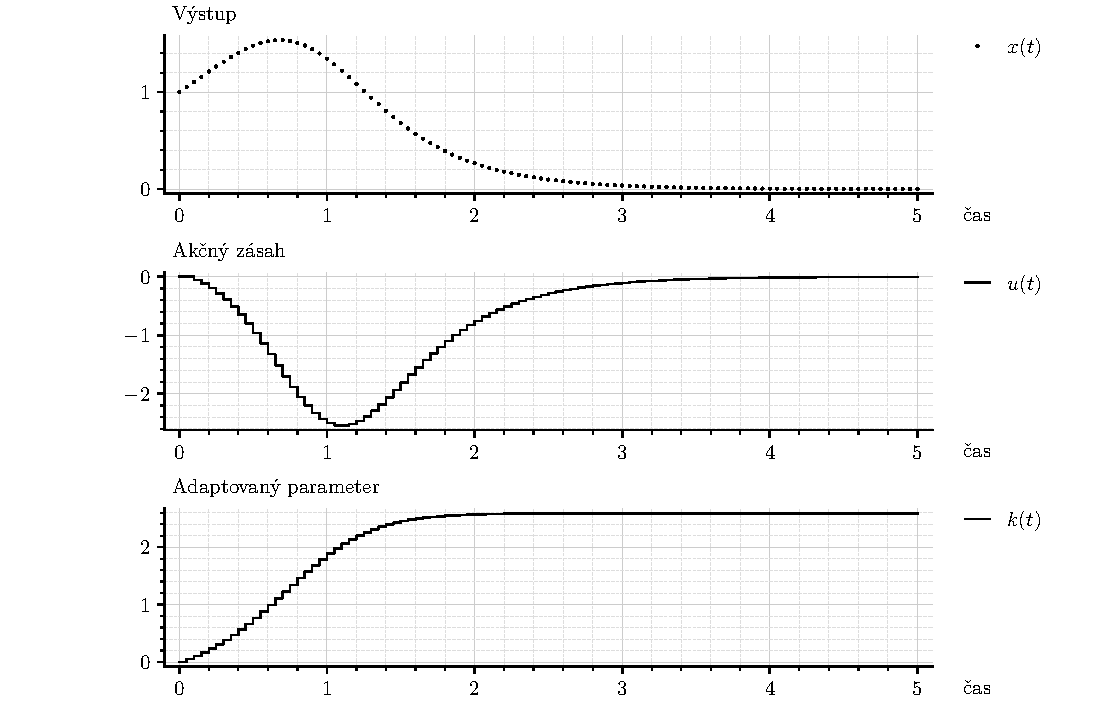
\includegraphics{figsc_ar02_f03_f01_0.pdf}
	}

    \vspace{-2mm}

    \figcaption{}

    \vspace{2mm}

    \label{figsc_ar02_f03_f01_0}

\end{centering}

\noindent
V čom je tá implementácia „realistická“? To je na diskusiu, ktorú tu autor neuvádza pretože je lenivý a naničhodný.






\end{document}
